\documentclass[11pt,a4paper]{article}

% ---------- Page layout ----------
\usepackage[margin=2.5cm]{geometry}
\usepackage{parskip}
\usepackage{microtype}

% ---------- Fonts / maths ----------
\usepackage[T1]{fontenc}
\usepackage{lmodern}
\usepackage{amsmath}
\usepackage{siunitx}
\sisetup{detect-all}

% ---------- Figures (vector only) ----------
\usepackage{graphicx}
\usepackage{float}
\usepackage[font=small,labelfont=bf]{caption}
\usepackage{subcaption}
\graphicspath{{figs/}{figures/}{../figures/}}

% ---------- Tables, links ----------
\usepackage{booktabs}
\newcommand{\rng}[2]{#1\,\textendash\,#2}
\usepackage{tabularx}
\usepackage[hidelinks]{hyperref}

% ---------- Code listings for the appendix ----------
\usepackage{xcolor}
\newcommand{\todo}[1]{\textcolor{red}{[#1]}} % draft notes; set to {} to hide before submitting
\usepackage{listings}
\lstset{
  language=Python,
  basicstyle=\ttfamily\footnotesize,
  keywordstyle=\color{blue!70!black},
  commentstyle=\color{green!40!black},
  stringstyle=\color{orange!70!black},
  numbers=left,
  numberstyle=\tiny\color{gray},
  breaklines=true,
  frame=single,
  columns=fullflexible,
  keepspaces=true,
  showstringspaces=false,
  literate={≈}{{$\approx$}}1 {’}{{'}}1 {—}{{---}}1 {–}{{--}}1 {μ}{{$\mu$}}1 {Δ}{{$\Delta$}}1 {×}{{$\times$}}1 {−}{{$-$}}1 {≥}{{$\ge$}}1
}

% ---------- Title info ----------
\title{Digital Signal Processing -- Assignment 2\\
       FIR Filters, Adaptive LMS Filtering, and Realtime ECG Peak Detection}
\author{
  Saad Aziz (GUID:\ 2917444A) \\
  William Chambers (GUID:\ 2906463C) \\[0.5em]
  University of Glasgow, School of Engineering
}
\date{\today}

\begin{document}
\maketitle

% =====================================================
\section{Recordings}
% =====================================================
\todo{State the lab recording setup: two ECG recordings saved as \texttt{ecg1.tsv} (primary recording analysed across Tasks 1--5, chosen for its clear P-wave visibility) and \texttt{ecg2.tsv} (partner's recording used exclusively in Task 5 to extract the QRS matched-filter template). Note that the signal is read from ADC channel 2 (column 8, 0-indexed) and the sampling rate is $f_s = 1/(t_1 - t_0) = \SI{250}{Hz}$ (Nyquist frequency $f_s/2 = \SI{125}{Hz}$). Reminder: only quote numbers the submitted code prints or plots ($M = 1000$ taps, group delay $\SI{1.998}{s}$, and $45$ heart rates at a mean of $\SI{92.0}{bpm}$); argue all other values visually from the figures.}

% =====================================================
\section{Task 1: Time and Frequency Analysis}
% =====================================================
\todo{Briefly state how the time vector $t = n / f_s$ and single-sided linear magnitude spectrum $|\mathrm{FFT}(\text{ecg})|/N$ up to $f_s/2$ were computed in \texttt{ecg\_plot.py} without using prohibited high-level functions such as \texttt{fftfreq}. Emphasise that the spectrum is plotted on a \textbf{linear axis} as required by the brief.}

\begin{figure}[H]
  \centering
  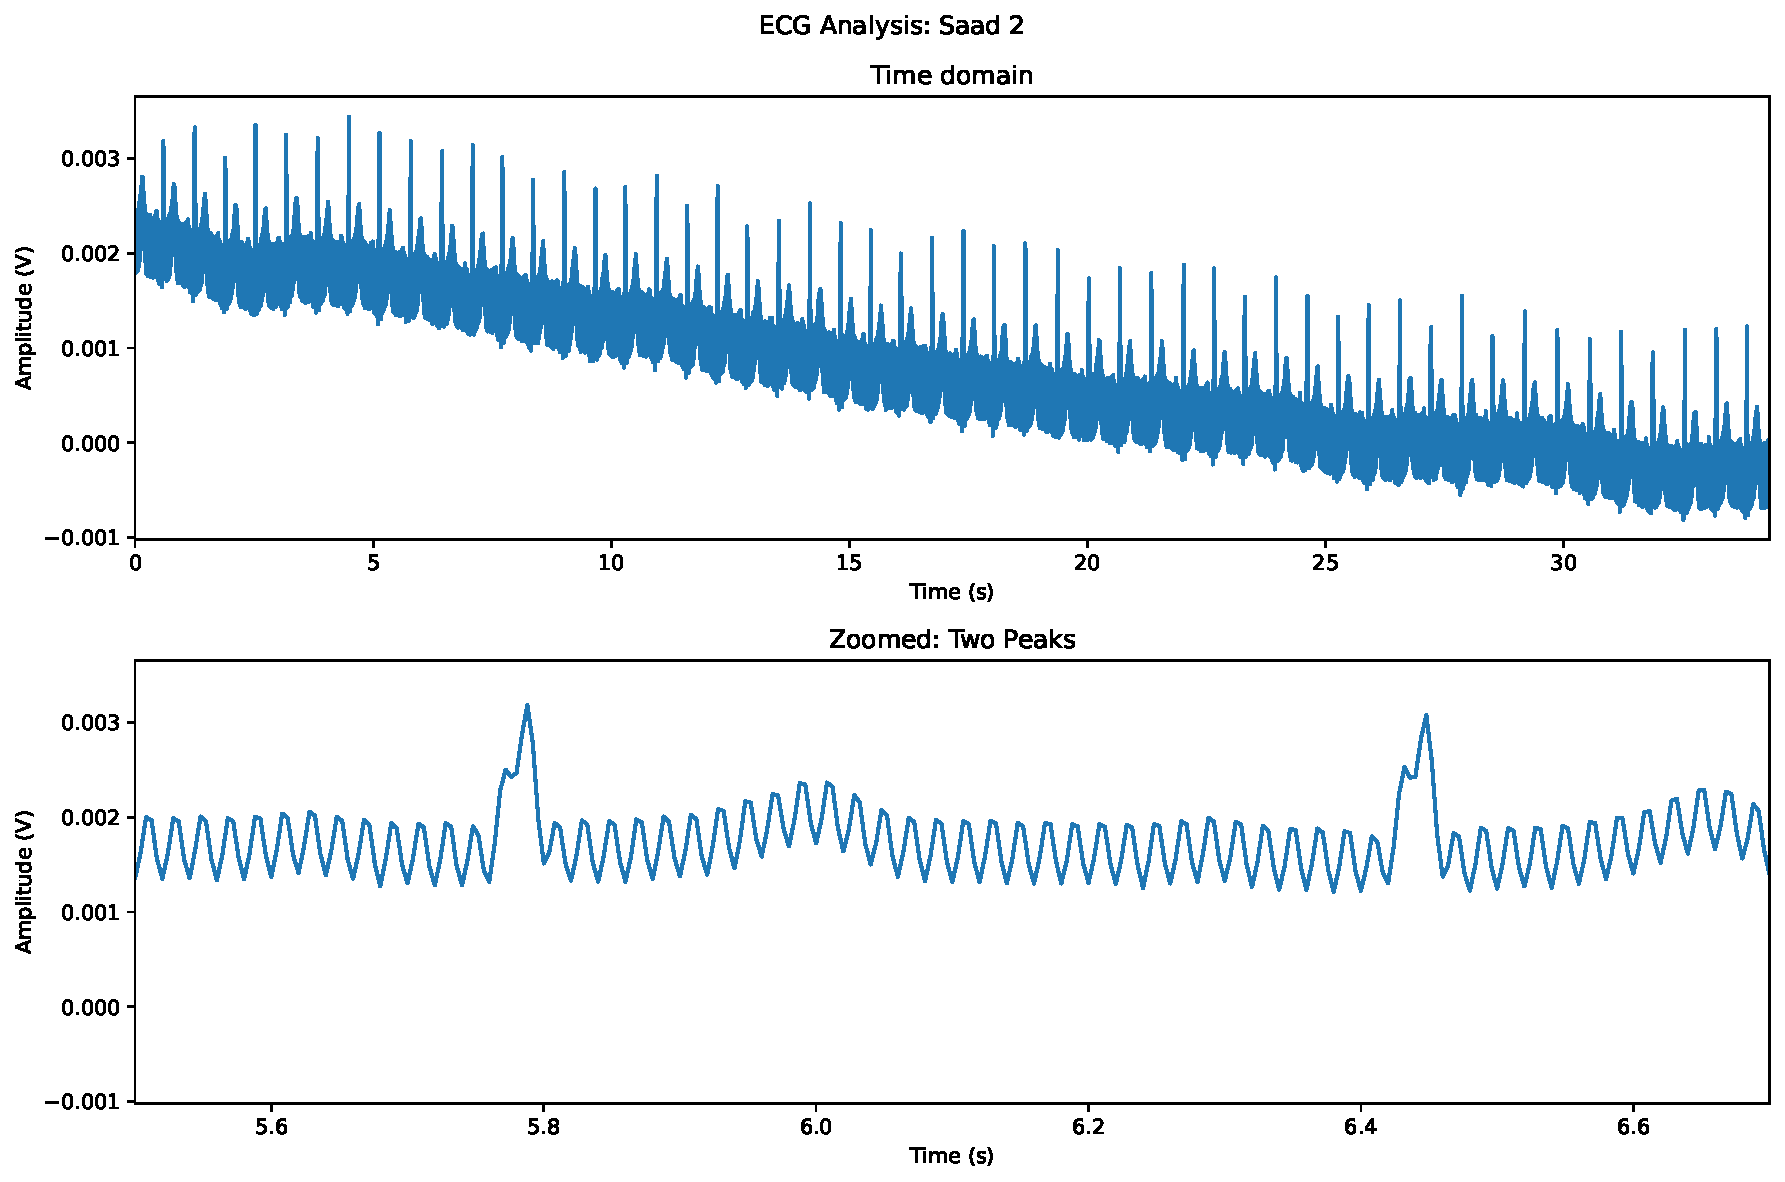
\includegraphics[width=\textwidth]{t1_time.pdf}
  \caption{Raw primary ECG (\texttt{ecg1.tsv}) in the time domain: (top) full recording showing downward baseline drift, and (bottom) zoomed window ($\rng{5.5}{6.7}\,\si{s}$) spanning two heartbeats with visible PQRST complexes and $\SI{50}{Hz}$ ripple. \todo{Annotate P, Q, R, S, T peaks in Inkscape if required.}}
  \label{fig:t1_time}
\end{figure}

\begin{figure}[H]
  \centering
  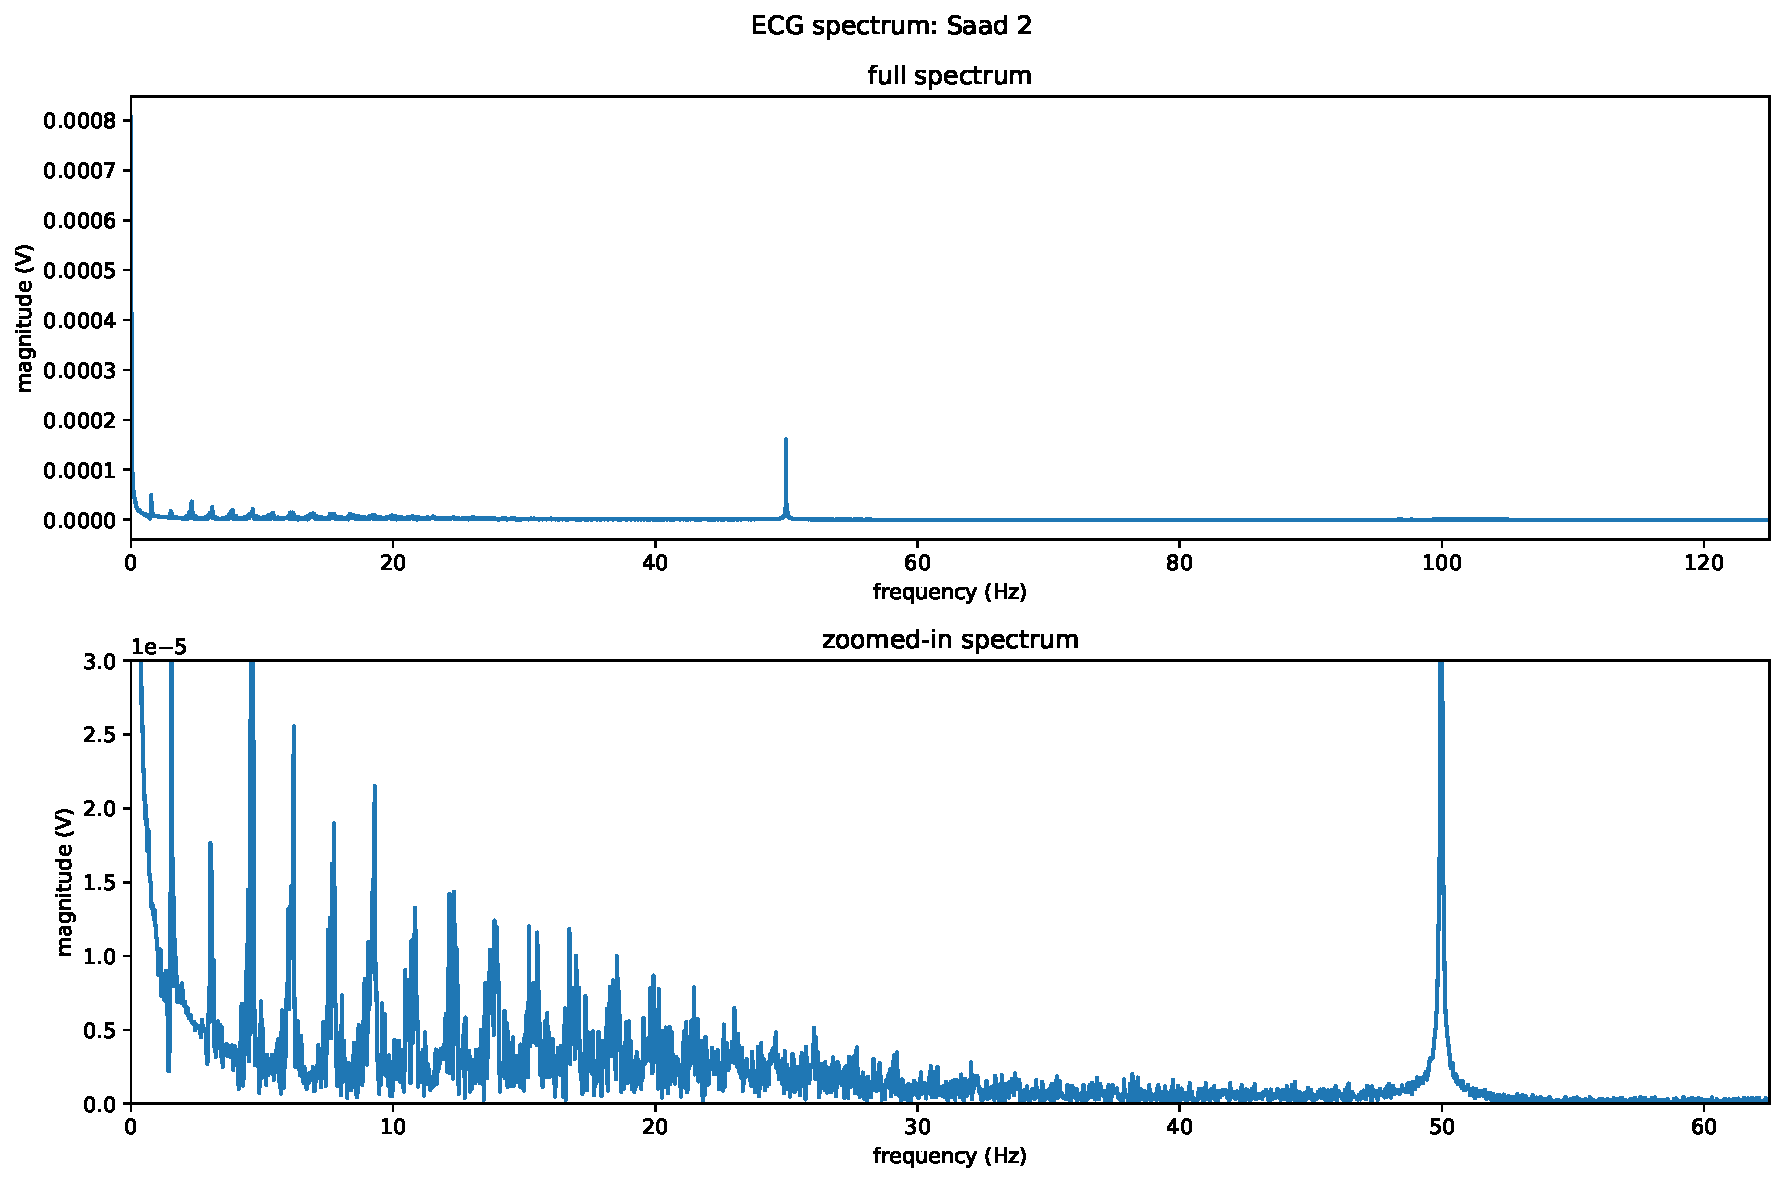
\includegraphics[width=\textwidth]{t1_freq.pdf}
  \caption{Single-sided linear frequency spectrum of \texttt{ecg1.tsv}: (top) full magnitude scale dominated by the $\SI{0}{Hz}$ DC/baseline spike and $\SI{50}{Hz}$ mains interference, and (bottom) zoomed magnitude scale (\rng{0}{\SI{3e-5}{V}}) revealing the fundamental heart-rate peak and its harmonic comb.}
  \label{fig:t1_freq}
\end{figure}

\paragraph{ECG signal and harmonics.}
\todo{From Fig.~\ref{fig:t1_time} (bottom), point out the two heartbeats in the $\rng{5.5}{6.7}\,\si{s}$ window (period $\approx \SI{0.66}{s}$, fundamental heart-rate frequency $\approx \SI{1.5}{Hz}$). In Fig.~\ref{fig:t1_freq} (bottom), identify the comb of equally spaced ECG harmonics at multiples of the heart rate that gradually fade out by about $\SI{40}{Hz}$.}

\paragraph{Noise and interferences.}
\todo{Identify each interference source from Figs.~\ref{fig:t1_time}--\ref{fig:t1_freq}:
(1) \textbf{DC offset and baseline wander:} the whole time trace drifts downwards over the recording (while the R-peaks keep the same height above the local baseline, proving it is baseline wander rather than signal attenuation), producing the large spike at $\SI{0}{Hz}$ and the lowest frequency bins ($<\SI{0.5}{Hz}$). Explicitly explain that \textbf{the DC bin is kept on purpose} because the $\SI{0}{Hz}$ spike represents the ADC offset plus baseline wander that our filter must remove---which is why a second, vertically zoomed spectrum is plotted;
(2) \textbf{$\SI{50}{Hz}$ mains interference:} visible as a regular sinusoidal ripple riding on the baseline in Fig.~\ref{fig:t1_time} (bottom) and as a sharp peak at $\SI{50}{Hz}$ in Fig.~\ref{fig:t1_freq}. Explicitly state that \textbf{no $\SI{100}{Hz}$ harmonic is visible} on the zoomed spectrum below the $\SI{125}{Hz}$ Nyquist frequency;
(3) \textbf{Broadband EMG / muscle noise:} any broadband muscle noise overlaps the $\rng{0.5}{40}\,\si{Hz}$ ECG harmonic band and therefore cannot be removed by frequency-selective filtering without distorting the heartbeat itself.}

\paragraph{Frequencies to remove.}
\todo{State and justify the two stopbands chosen for Task 2:
(1) $\rng{0}{0.5}\,\si{Hz}$ to remove the DC offset and slow respiration/movement baseline wander while staying well below the $\approx \SI{1.5}{Hz}$ fundamental heart rate;
(2) $\rng{45}{125}\,\si{Hz}$ to remove the $\SI{50}{Hz}$ mains interference and all high-frequency noise up to Nyquist. Justify \textbf{why $\SI{45}{Hz}$ was chosen}: in Fig.~\ref{fig:t1_freq} (bottom), the ECG harmonics fade by about $\SI{40}{Hz}$ and the $\SI{50}{Hz}$ interference skirt begins at about $\SI{48}{Hz}$, so placing the cut-off at $\SI{45}{Hz}$ centres the filter's transition band in that natural spectral gap.}

% =====================================================
\section{Task 2: FIR Filter Coefficient Design}
% =====================================================

\paragraph{Number of coefficients.}
\todo{Explain how \texttt{fir\_design(sample\_rate, ranges)} in \texttt{fir\_design.py} automatically determines the tap count $M = 1000$:
(1) It finds the narrowest stopband width $\Delta f_{\min} = \min(\text{high} - \text{low})$, which is $\rng{0}{0.5}\,\si{Hz}$ ($\Delta f_{\min} = \SI{0.5}{Hz}$);
(2) It halves this width to set the frequency bin spacing $\delta f = \Delta f_{\min}/2 = \SI{0.25}{Hz}$ so that even the narrowest stopband spans at least two frequency bins;
(3) It computes $M = \lfloor f_s / \delta f \rfloor = 250 / 0.25 = 1000$, and enforces even parity (\texttt{M += M \% 2}) so the impulse response splits into two equal halves of length $M/2$ during the causal shift;
(4) Discuss the delay trade-off: a linear-phase FIR filter has a group delay of $(M-1)/2 \text{ samples} = \SI{1.998}{s}$. For a fixed $M$, increasing $f_s$ reduces the delay; however, for a fixed frequency resolution $\delta f$, the delay $\approx (M-1)/(2f_s) \approx 1/(2\,\delta f)$ is fundamentally set by how close to DC ($\SI{0.5}{Hz}$) the filter must cut.}

\paragraph{IFFT coefficient calculation and edge cases.}
\todo{Walk through the design steps in \texttt{fir\_design.py}:
(1) \textbf{Folded frequency axis and edge cases:} the bin frequencies $f_k = k\,f_s / M$ are folded via \texttt{f = np.minimum(f, sample\_rate - f)} so bin $M-k$ is assigned the same frequency as bin $k$. This guarantees conjugate symmetry and handles the \textbf{DC and Nyquist edge cases} automatically: bin $0$ is labelled $\SI{0}{Hz}$ (DC) and bin $M/2$ is labelled $f_s/2 = \SI{125}{Hz}$ (Nyquist);
(2) \textbf{Ideal response:} $H[k]$ is initialised to $1$ everywhere (passband) and set to $0$ for every bin falling within the target stopband ranges ($\rng{0}{0.5}\,\si{Hz}$ and $\rng{45}{125}\,\si{Hz}$);
(3) \textbf{IFFT and half-swap:} applying \texttt{np.real(ifft(H))} yields the zero-phase impulse response (the imaginary part vanishes because $H$ is symmetric). Swapping the first and second halves (\texttt{h\_shift}) centres the impulse response at $M/2$ to make the filter causal;
(4) \textbf{Windowing:} multiplying by a Hamming window (\texttt{np.hamming(M)}) tapers the truncated impulse response tails to suppress Gibbs phenomenon passband/stopband ringing.}

\begin{figure}[H]
  \centering
  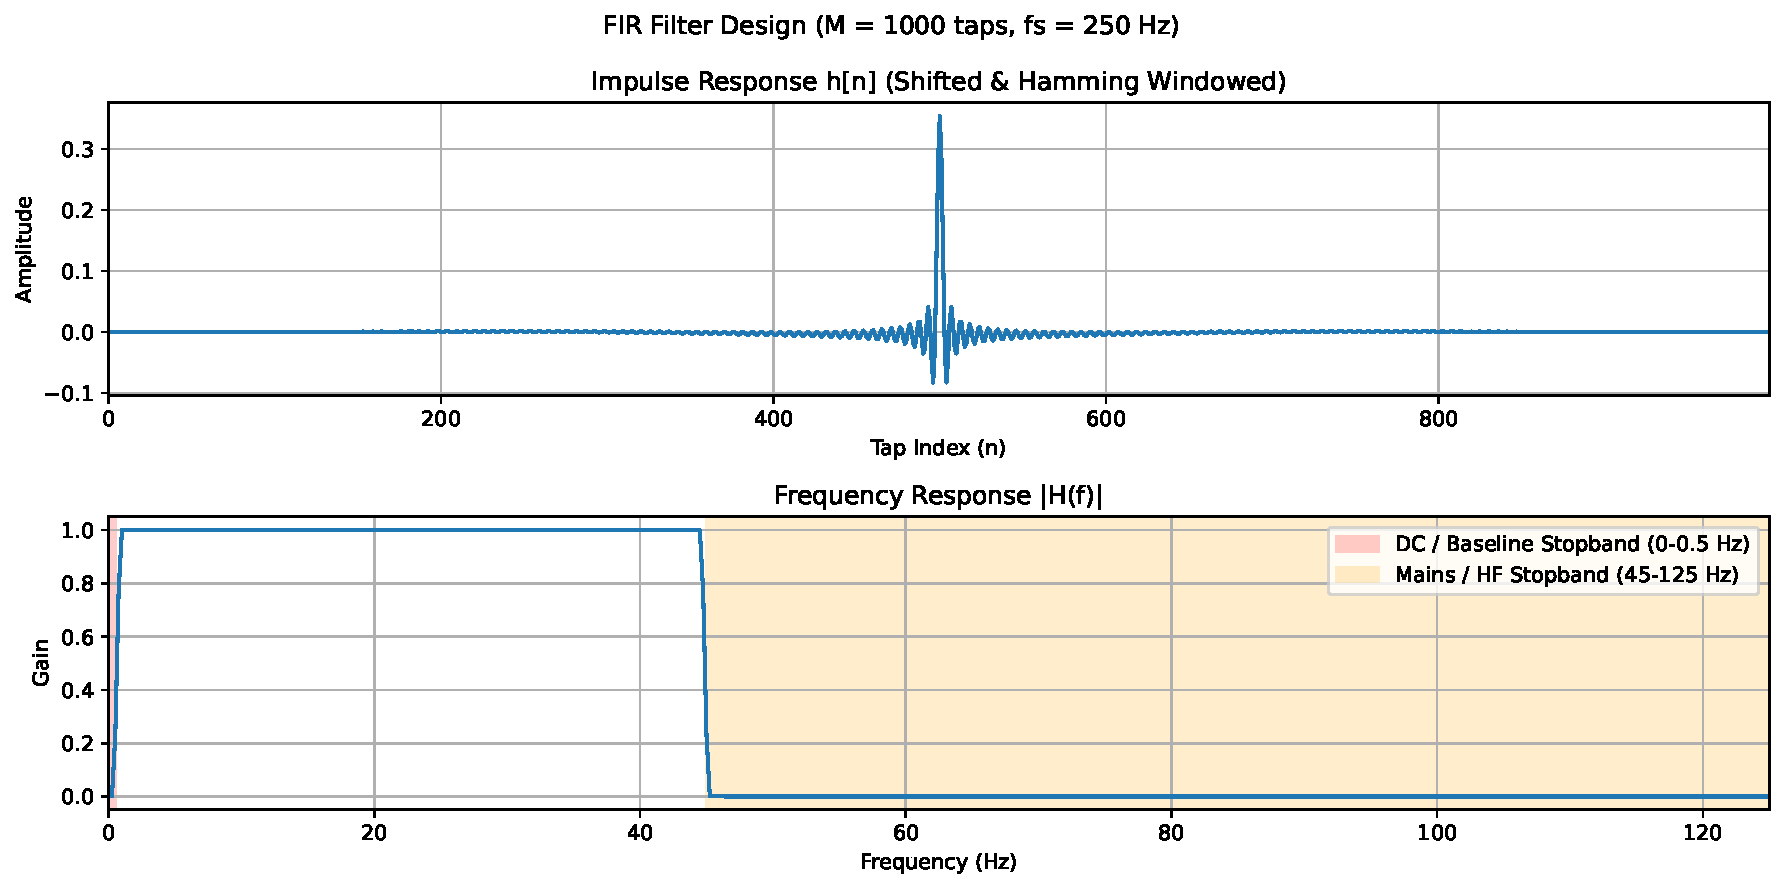
\includegraphics[width=\textwidth]{t2_coeffs.pdf}
  \caption{Designed FIR filter ($M = 1000$ taps, $f_s = \SI{250}{Hz}$): (top) shifted and Hamming-windowed impulse response $h[n]$ centred at $M/2 = 500$, and (bottom) frequency response magnitude $|H(f)|$ showing the $\rng{0}{0.5}\,\si{Hz}$ and $\rng{45}{125}\,\si{Hz}$ stopbands.}
  \label{fig:t2_coeffs}
\end{figure}

% =====================================================
\section{Task 3: Realtime FIR Filtering}
% =====================================================

\paragraph{Ring-buffer implementation.}
\todo{Explain \texttt{class FIRfilter} in \texttt{fir\_filter.py}:
(1) \texttt{\_\_init\_\_(self, \_coefficients)} stores the $M$ tap weights, allocates a zero-initialised delay buffer of length $M$, and sets the write pointer \texttt{self.offset = 0};
(2) \texttt{dofilter(self, v)} takes a single scalar input sample $x[n]$ and returns a single scalar output $y[n] = \sum_{m=0}^{M-1} h[m]\,x[n-m]$;
(3) Emphasise that \textbf{a circular ring buffer is used instead of \texttt{np.roll} or array shifting}: nothing in the buffer is shifted in memory (which the brief penalises). Only the write pointer \texttt{self.offset} moves forward (wrapping to $0$ at $M-1$), and the convolution sum is vectorised as two sliced dot products across the wrap-around boundary (\texttt{coefficients[:k]} with \texttt{buffer[offset::-1]} and \texttt{coefficients[k:]} with \texttt{buffer[:offset:-1]}).}

\paragraph{Filtered ECG results.}
\todo{Discuss the realtime simulation in \texttt{fir\_realtime\_sim.py} (Fig.~\ref{fig:t3_filtered}):
(1) \textbf{Start-up transient:} the first $M = 1000$ samples ($\approx \SI{4}{s}$) exhibit a start-up transient while the zero-initialised ring buffer fills with the DC-offset ECG signal, after which the baseline sits flat on $\SI{0}{V}$;
(2) \textbf{Delay-aligned PQRST verification:} after aligning the filtered trace by the $(M-1)/2 = \SI{1.998}{s}$ group delay (labelled $\SI{2.0}{s}$ in the plot legend), the zoomed comparison in Fig.~\ref{fig:t3_filtered} (middle) confirms that the $\SI{50}{Hz}$ ripple is completely eliminated while the P, Q, R, S, and T waves remain intact and undistorted;
(3) \textbf{Spectral verification:} the filtered spectrum (bottom) confirms complete attenuation below $\SI{0.5}{Hz}$ and above $\SI{45}{Hz}$ while preserving the ECG harmonic comb.}

\begin{figure}[H]
  \centering
  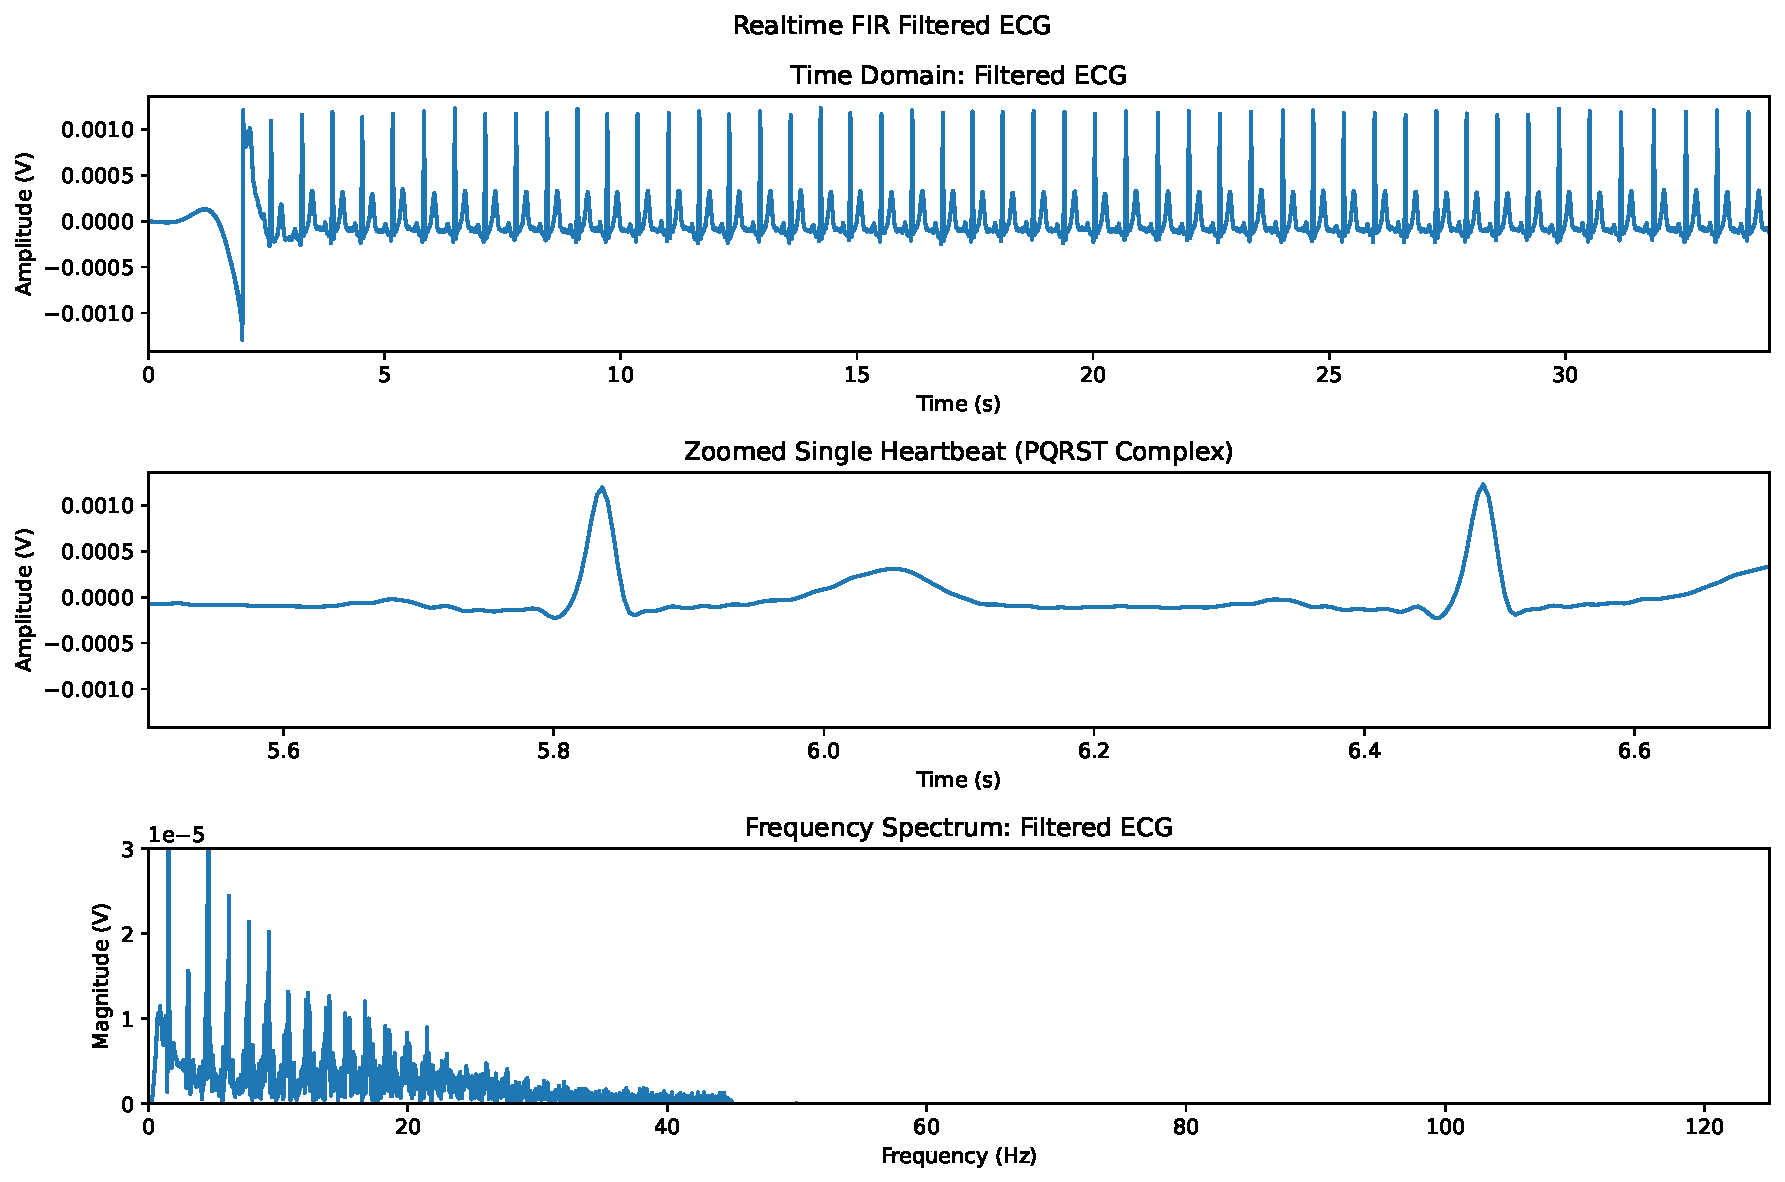
\includegraphics[width=\textwidth]{t3_filtered.pdf}
  \caption{Task 3 sample-by-sample FIR filtering of \texttt{ecg1.tsv} ($M = 1000$, group delay $\SI{1.998}{s}$): (top) full time-domain trace, (middle) zoomed heartbeat window ($\rng{5.5}{6.7}\,\si{s}$) verifying intact PQRST morphology, and (bottom) linear frequency spectrum.}
  \label{fig:t3_filtered}
\end{figure}

% =====================================================
\section{Task 4: Adaptive LMS Filter}
% =====================================================

\paragraph{Implementation and series architecture.}
\todo{Explain \texttt{doFilterAdaptive(self, signal, noise, learningRate)} in \texttt{fir\_filter.py} and the two-stage design in \texttt{lms\_filter.py}:
(1) \textbf{Method operation:} on each scalar step, \texttt{doFilterAdaptive} saves the current write pointer \texttt{read\_idx = self.offset}, passes the scalar reference \texttt{noise} $x[n]$ through \texttt{self.dofilter(noise)} to form the interference estimate $y[n]$, computes the cleaned ECG error $e[n] = \text{signal} - y[n]$, and updates the tap weights in-place via $w_m \leftarrow w_m + \mu\,e[n]\,x[n-m]$ using the same two-slice ring-buffer indexing;
(2) \textbf{Two cancellers in series:} a 1-tap DC/baseline canceller (constant reference $1.0$, $\mu_{\text{dc}} = 0.0125$) is placed in series before a 10-tap $\SI{50}{Hz}$ canceller (sine reference $\sin(2\pi \cdot 50\,i / f_s)$, $\mu_{\text{lms}} = 0.01$, which requires multiple taps to adjust both amplitude and phase of the $\SI{50}{Hz}$ sinusoid);
(3) \textbf{Qualitative justification of the design change:} state that a single LMS filter with a combined reference ($1.0 + \sin(\dots)$) was tried first, but its DC term adapted too quickly and acted as a high-pass filter that visibly flattened the slow P and T waves. Splitting into two series cancellers decouples the slow baseline adaptation from the fast $\SI{50}{Hz}$ cancellation.}

\paragraph{Comparison with the Task 3 FIR filter.}
\todo{Compare the adaptive LMS output against the Task 3 fixed FIR output using Fig.~\ref{fig:t4_compare}:
(1) \textbf{Waveform overlap:} once the Task 3 FIR trace is shifted back by its $\SI{1.998}{s}$ delay, the zoomed heartbeats overlap closely with intact PQRST waves;
(2) \textbf{Frequency-domain difference:} the LMS filter acts as a narrow notch at DC and $\SI{50}{Hz}$---it retains frequency content above $\SI{45}{Hz}$ and leaves a small $\SI{50}{Hz}$ spectral residual---whereas the Task 3 FIR filter removes everything from $\rng{45}{125}\,\si{Hz}$, so the two filters do not perform quite the same job;
(3) \textbf{Delay and settling:} the LMS filter has \textbf{no $\SI{2}{s}$ group delay} (only the FIR trace requires delay alignment) and uses only $1 + 10 = 11$ taps versus $M = 1000$ taps, while the DC canceller visibly settles to $\SI{0}{V}$ over the first few seconds of the recording.}

\begin{figure}[H]
  \centering
  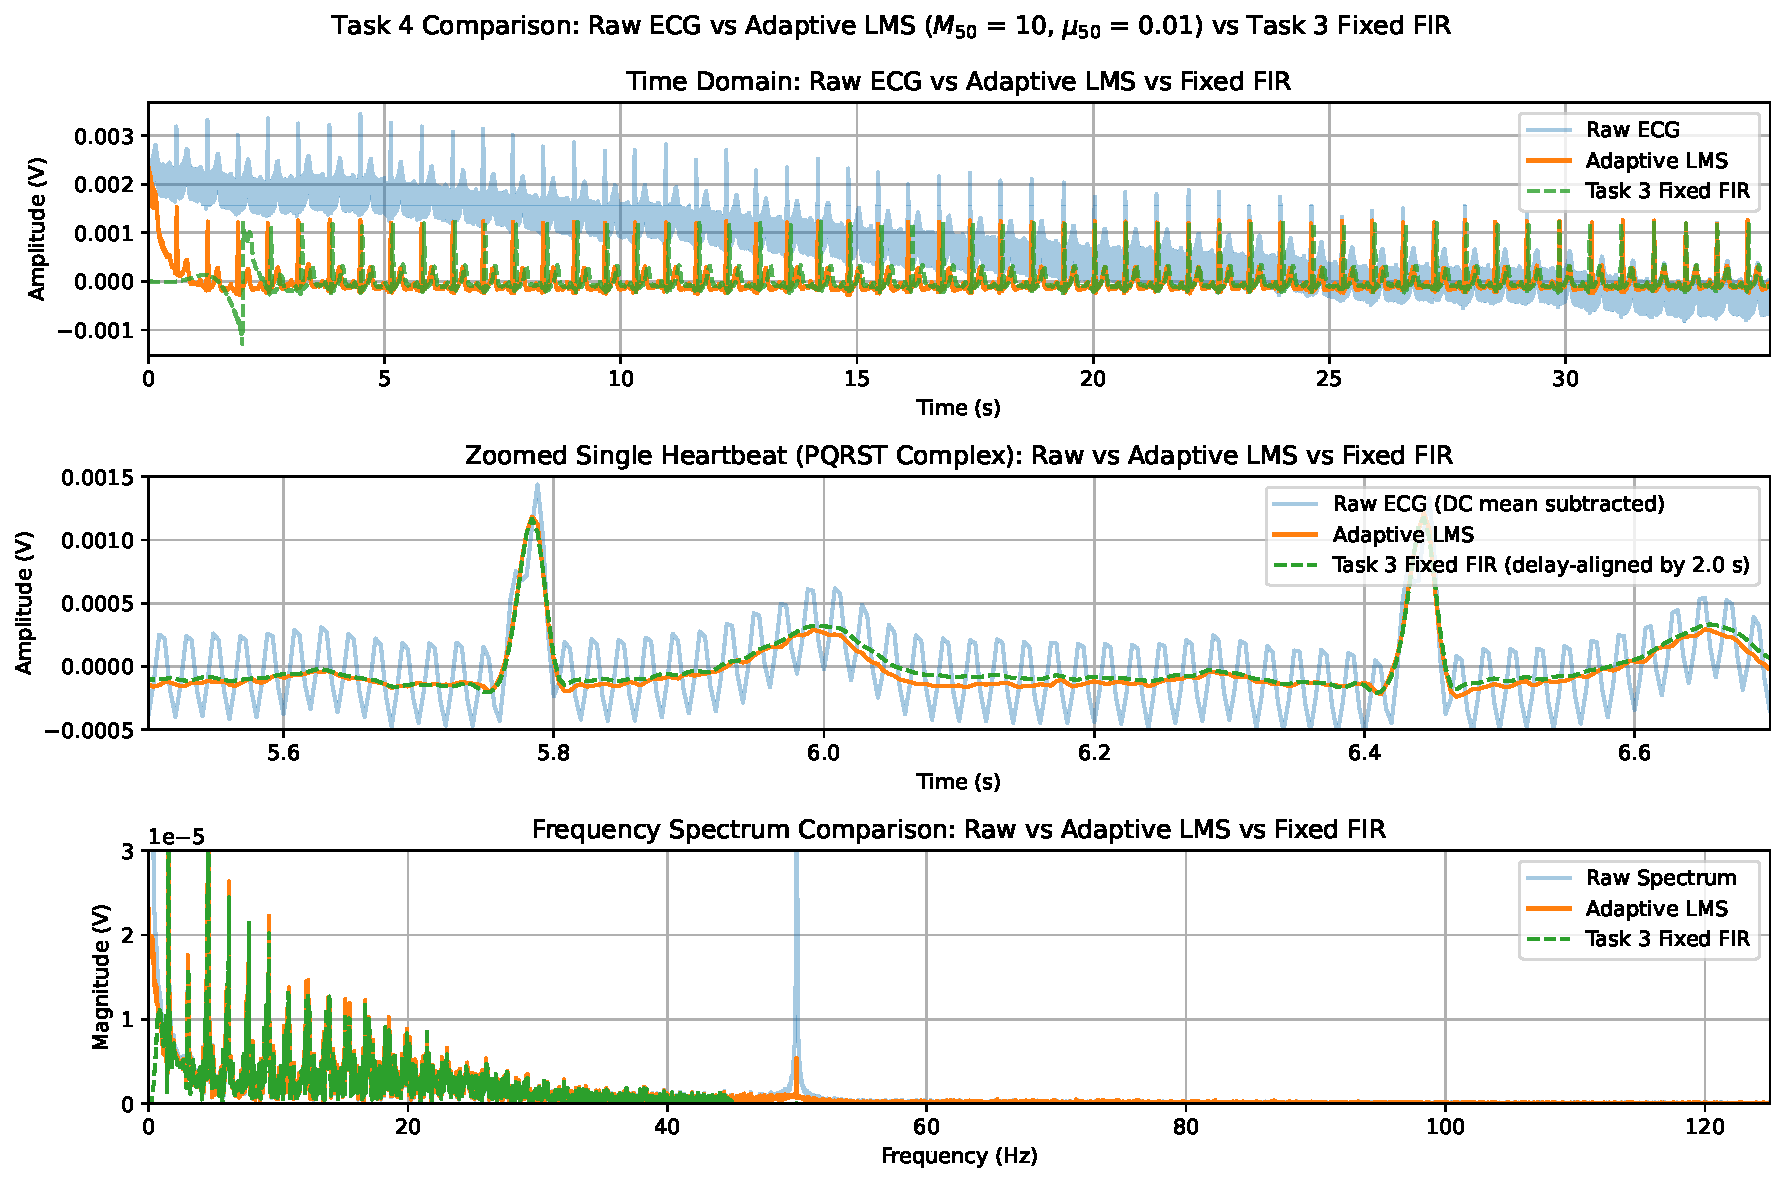
\includegraphics[width=\textwidth]{t4_compare.pdf}
  \caption{Comparison between the Task 3 fixed FIR filter ($M = 1000$) and the Task 4 two-stage adaptive LMS filter ($M_{\text{DC}} = 1, \mu_{\text{dc}} = 0.0125$; $M_{\text{LMS}} = 10, \mu_{\text{lms}} = 0.01$) across (top) full time domain, (middle) delay-aligned zoomed heartbeat, and (bottom) linear frequency spectrum.}
  \label{fig:t4_compare}
\end{figure}

% =====================================================
\section{Task 5: ECG Heartbeat Detection}
% =====================================================

\paragraph{Template extraction and matched filter.}
\todo{Explain the matched filter design in \texttt{heartbeat.py}:
(1) \textbf{Template source:} the partner's recording (\texttt{ecg2.tsv}) is first cleaned sample-by-sample using the exact same Task 2 FIR filter ($h$) so that both the template and the test ECG have the same filtered shape. A 25-sample QRS segment ($\pm 12$ samples around $R = 2576$, i.e.\ $\pm \SI{48}{ms}$) is sliced \emph{after} the cleaning filter's 1000-sample buffer has completely filled (Fig.~\ref{fig:t5_detection}, top);
(2) \textbf{Time reversal:} the matched filter coefficients are set to the time-reversed template (\texttt{np.flip(template)}), because an FIR filter multiplies its first coefficient with the newest input sample (convolution), which equals cross-correlation when the template is reversed in time---avoiding prohibited functions like \texttt{correl} or \texttt{conv};
(3) \textbf{Squaring:} the matched filter output is squared (\texttt{** 2}) at each sample so that it is strictly positive and the tall R-peak correlation spikes are strongly emphasised relative to smaller Q/S/T side lobes.}

\paragraph{Thresholding, warm-up, and physiological heuristics.}
\todo{Explain the realtime R-peak detector and heuristics in \texttt{heartbeat.py} (Fig.~\ref{fig:t5_detection}, bottom):
(1) \textbf{Warm-up transient exclusion:} the first $\texttt{TRANSIENTS} = \text{len}(h) + \text{len}(\text{template}) = 1000 + 25 = 1025$ samples ($\approx \SI{4.1}{s}$, shaded grey) are ignored because both cascaded filters in series (cleaning FIR + matched FIR) must fill their ring buffers before producing valid outputs;
(2) \textbf{Threshold justification ($\SI{1.5e-11}{V^4}$):} chosen directly from Fig.~\ref{fig:t5_detection} (bottom), sitting with wide margin below all true R-peak spikes ($\ge \SI{2.1e-11}{V^4}$) and well above the secondary side spikes ($\approx \SI{0.8e-11}{V^4}$);
(3) \textbf{Rising-edge detection:} a beat is triggered only when the squared output crosses upward through the threshold (\texttt{out[i] > THRESHOLD and out[i-1] <= THRESHOLD}), ensuring each peak is counted once;
(4) \textbf{Heuristics:} two rules filter the momentary heart rate $\mathrm{HR} = 60\,f_s / (n_{\text{peak}} - n_{\text{last}})$: first, physiological bounds of $\rng{30}{200}\,\si{bpm}$ (established from discussion with a physiology student); second, a beat-to-beat consistency check requiring each new rate to fall within $\pm 20\%$ ($\rng{0.80}{1.20}\times$) of the previous accepted rate, which automatically rejects missed beats ($-50\%$ apparent rate) and double detections ($+100\%$ apparent rate).}

\begin{figure}[H]
  \centering
  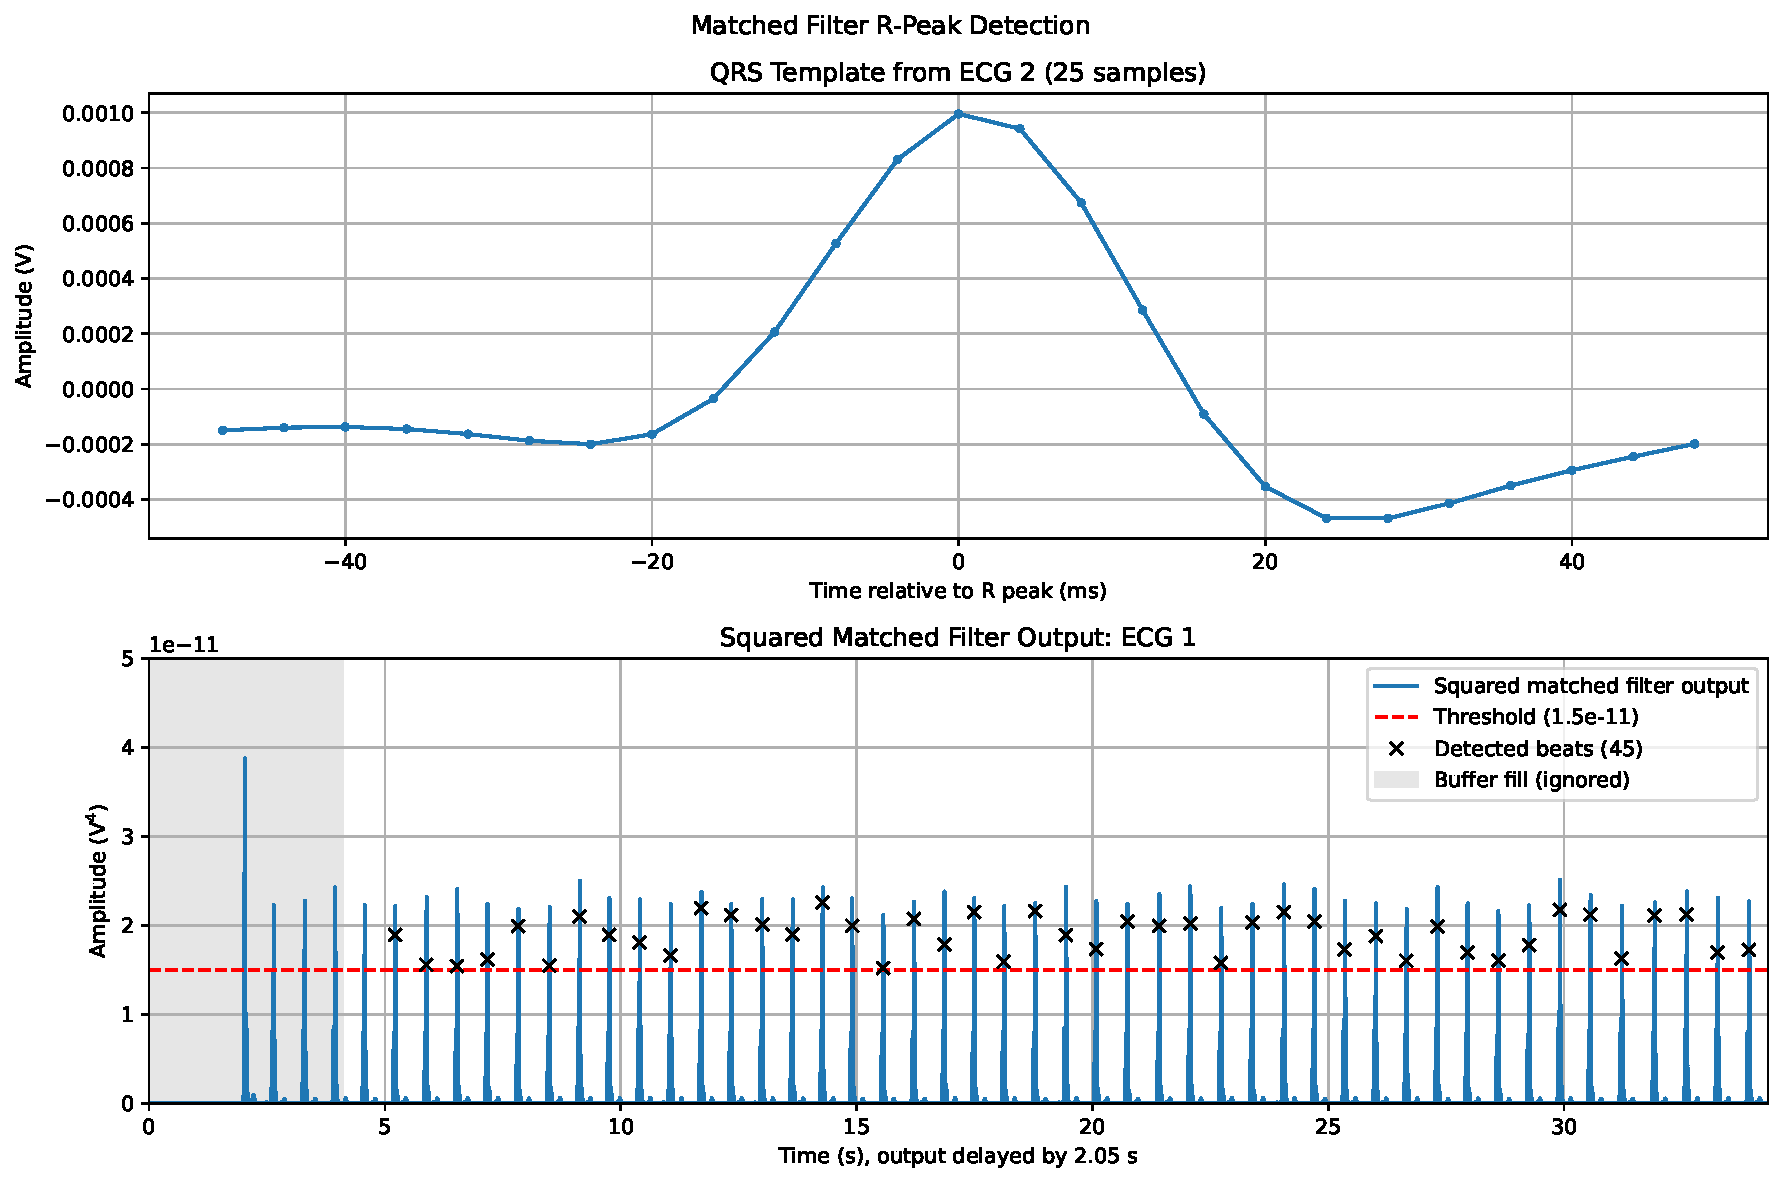
\includegraphics[width=\textwidth]{t5_detection.pdf}
  \caption{Task 5 matched-filter R-peak detection: (top) 25-sample QRS template extracted from cleaned \texttt{ecg2.tsv} around sample $R = 2576$, and (bottom) squared matched-filter output on \texttt{ecg1.tsv} showing the $\SI{1025}{sample}$ buffer-fill exclusion zone, the $\SI{1.5e-11}{V^4}$ threshold, and the $45$ accepted beat intervals.}
  \label{fig:t5_detection}
\end{figure}

\paragraph{Momentary heart rate analysis.}
\todo{Discuss the momentary heart-rate plot in Fig.~\ref{fig:t5_heartrate}:
(1) \textbf{46 beats $\to$ 45 heart rates:} the detector finds $46$ valid R-peaks after the warm-up period, yielding $45$ inter-beat intervals and a printed mean heart rate of $\SI{92.0}{bpm}$ (the first detected beat has no preceding beat to form an interval, so it produces no rate and is not plotted);
(2) \textbf{Heart-rate variability (HRV):} the momentary heart rate fluctuates naturally by a few bpm from beat to beat around $\SI{92.0}{bpm}$. Explain that this is normal physiological heart-rate variability (respiratory sinus arrhythmia, where heart rate rises slightly during inhalation and falls during exhalation) rather than detection jitter;
(3) \textbf{Effect of filter delay:} the combined linear-phase delay of the cleaning filter ($\SI{1.998}{s}$) and matched filter ($\SI{0.048}{s}$) is $\SI{2.046}{s}$ (displayed as $\SI{2.05}{s}$). Because every detected beat is delayed by the exact same constant offset, the time intervals between beats---and hence the momentary heart rates---are completely unaffected (and the plotted time axis is shifted back by \texttt{delay} to align with the raw ECG).}

\begin{figure}[H]
  \centering
  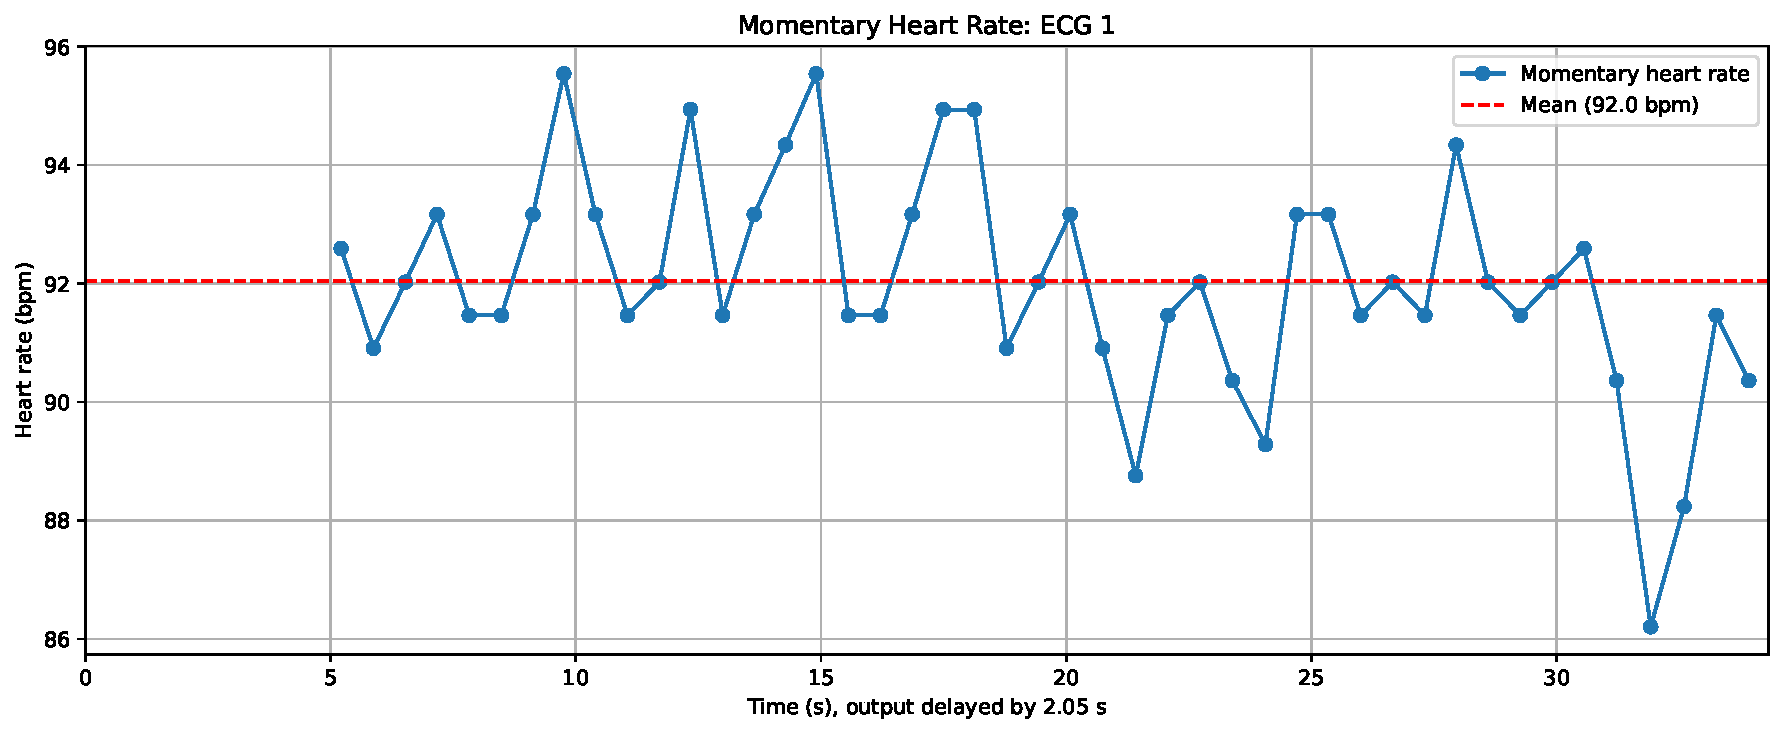
\includegraphics[width=\textwidth]{t5_heartrate.pdf}
  \caption{Momentary heart rate over time for \texttt{ecg1.tsv} across $45$ beat-to-beat intervals (mean heart rate $\SI{92.0}{bpm}$), delay-aligned to the input ECG timeline.}
  \label{fig:t5_heartrate}
\end{figure}

%------------------------------------------------------------------------------------------------------------------------------------------------------
\pagebreak
% =====================================================
\appendix

\section{Acknowledgement of GenAI Use}
% =====================================================
\textbf{Tools:}
\todo{State exact tool name, version, and publisher, e.g.\ Claude Opus 4.5 / 5.5 (Anthropic).}\\
\textbf{Use:}
\todo{State how GenAI was used (e.g.\ suggesting the folded frequency axis \texttt{np.minimum(f, sample\_rate - f)} in Task 2 and assisting with matplotlib formatting for the momentary heart-rate plot in Task 5) and what work the team contributed directly (lab ECG recordings, spectral diagnosis and cut-off selection, tap-count derivation, ring-buffer FIR and two-stage series LMS implementation, matched-filter template extraction and heuristic design, and writing the report).}

\section{Usage Instructions}
% =====================================================
All scripts use platform-independent relative paths (\texttt{pathlib.Path}) and require \texttt{numpy}, \texttt{scipy}, and \texttt{matplotlib}. After unzipping the submission archive, run each script directly from a terminal in the unzipped directory:
\begin{verbatim}
python ecg_plot.py
python fir_realtime_sim.py
python lms_filter.py
python heartbeat.py
\end{verbatim}

\section{Python Code}
% =====================================================

\subsection{support\_funcs.py}
\lstinputlisting{../support_funcs.py}

\subsection{ecg\_plot.py}
\lstinputlisting{../ecg_plot.py}

\subsection{fir\_design.py}
\lstinputlisting{../fir_design.py}

\subsection{fir\_filter.py}
\lstinputlisting{../fir_filter.py}

\subsection{fir\_realtime\_sim.py}
\lstinputlisting{../fir_realtime_sim.py}

\subsection{lms\_filter.py}
\lstinputlisting{../lms_filter.py}

\subsection{heartbeat.py}
\lstinputlisting{../heartbeat.py}

\end{document}
